\documentclass[
  12pt,				    % tamanho da fonte
  openright,			% capítulos começam em pág ímpar (insere página vazia caso preciso)
  oneside,			  % para impressão em recto e verso. Oposto a oneside
  a4paper,			  % tamanho do papel. 
  chapter=TITLE,  % títulos de capítulos convertidos em letras maiúsculas
  section=TITLE,  % títulos de seções convertidos em letras maiúsculas
  english,			  % idioma adicional para hifenização
  french,				  % idioma adicional para hifenização
  spanish,			  % idioma adicional para hifenização
  brazil				  % o último idioma é o principal do documento
]{iftex}

%% Arial: 
% Para usar times-new-roman, comente as três linhas abaixo
\usepackage{helvet}
\renewcommand{\familydefault}{\sfdefault}
\renewcommand{\ABNTEXchapterfont}{\bfseries}

\usepackage{easyReview} % Comandos para revisar o texto

%% Macros de dados do documento
\autor{Autor do projeto}
\titulo{Título do projeto}
\instituicao{Instituto federal do espírito santo}
\curso{Curso de Engenharia Elétrica}
\local{Vitória}
\data{2018}

\tipotrabalho{Trabalho de Graduação}
\preambulo{Trabalho de Conclusão de Curso apresentado à Coordenadoria do Curso de Engenharia Elétrica do
Instituto Federal de Educação, Ciência e Tecnologia do Espírito Santo, como requisito parcial para a obtenção do título de Engenheiro Eletricista.}
\orientador[Orientador][Prof. Dr.]{Beltrano}[de Tal]{Instituto Federal do Espírito Santo}
\coorientador[Coorientadora][Profa. Dra.]{Beltrana}[de Tal]{Instituto Federal do Espírito Santo}

\palavraschave{Palavra Chave 1}[Palavra Chave 2][Palavra Chave 3][Palavra Chave 4][Palavra Chave 5][Palavra Chave 6]

\cutter{X999y}
\cdd{000.00}

\begin{document}

  % Seleciona o idioma do documento
  \selectlanguage{brazil}
  
  % Insere a pasta onde estão contidas as figuras
  \graphicspath{{figuras/}}

  % --------------------------------------------------- %
  % ELEMENTOS PRE-TEXTUAIS %
  % --------------------------------------------------- %

  \pretextual

  % CAPA E CONTRA-CAPA
  \imprimircapa
  \imprimirfolhaderosto
  \imprimirfichacatalografica
   
  % FICHA CATALOGRAFICA ==> Adicione com anexo
	% \begin{fichacatalografica}
  % \includepdf{fig_ficha_catalografica.pdf}
	% \end{fichacatalografica}

  % FOLHA DE APROVAÇÃO
  % \orientadori{Prof. Dr. Beltrano de Tal}{Instituto Federal do Espírito Santo}{Orientador}
  % \orientadorii{Profa. Dra. Beltrana de Tal}{Instituto Federal do Espírito Santo}{Coorientadora}
  \examinadori{Profa. Dra. Fulana de Tal}{Instituto Federal do Espírito Santo}{Examinadora}
  \examinadorii{Prof. Dr. Cicrano de Tal}{Instituto Federal do Espírito Santo}{Examinador}
  \approvaldate{01}{Dezembro}{2018}

  \imprimiraprovacao

  % DEDICATÓRIA
  \imprimirdedicatoria{A dedicatória é um elemento opcional. Contém o oferecimento do trabalho adeterminada pessoa ou a pessoas (ASSOCIAÇÃO BRASILEIRA DE NORMAS TÉCNICAS, 2011b).}
    
  % AGRADECIMENTOS
  \begin{agradecimentos}
    A um elemento opcional. Localiza-se após a folha de aprovação e deve ser dirigido àqueles que realmente contribuíram, de maneira relevante,para a elaboração do trabalho. Deve-se utilizar uma linguagem simples (ASSOCIAÇÃO BRASILEIRA DE NORMAS TÉCNICAS, 2011b).
  \end{agradecimentos}
  
  % EPIGRAFE
  \begin{epigrafe}
    \vspace*{\fill}
    \begin{center}
      \textbf{Epigrafe:} É um elemento opcional. É uma citação relacionada ao assunto do trabalho desenvolvido, seguida da indicação de autoria (ASSOCIAÇÃO BRASILEIRA DE NORMAS TÉCNICAS, 2011b).   Deve-se seguir as regras do uso da citação NBR 10.520/2002. 
    \end{center}
  \end{epigrafe}
  
  % RESUMO - PT/EN
  % RESUMO - PT
\begin{resumo}
  \vspace{-15pt}
  
  É a apresentação concisa e abreviada do conteúdo de um texto, do qual destacam-se as informações essenciais e os elementos de maior relevância. Em um resumo, o texto deve ser significativo, explicando o tema principal do documento, o objetivo, a metodologia, os resultados e as conclusões do trabalho. Resumir um texto consiste em fazer a exposição sucinta de um assunto, tendo em vista permitir ao leitor conhecer as informações mais importantes sobre este para, então,poder decidir sobre a conveniência de consultar ou não o texto integralmente (ASSOCIAÇÃO BRASILEIRA DE NORMAS TÉCNICAS, 2003a).

  \textbf{De 150 a 500 palavras – os resumos de trabalhos acadêmicos (teses, dissertações e outros) e relatórios técnico-científicos}

  \textbf{Palavras-chave}: Palavra-chave 1; Palavra-chave 2; ...; Palavra-chave N.
\end{resumo}

% RESUMO - EN
\begin{resumo}[Abstract]
  \vspace{-15pt}
  
  \begin{otherlanguage*}{english}
  Enter the abstract here!
  
  \textbf{Keywords}: latex. abntex. text editoration.
\end{otherlanguage*}
\end{resumo}

  % LISTA DE FIGURAS
  \pdfbookmark[0]{\listfigurename}{lof}
  \listoffigures*
  \cleardoublepage

  % LISTA DE TABELAS
  \pdfbookmark[0]{\listtablename}{lot}
  \listoftables*
  \cleardoublepage

  % LISTA DE QUADROS
  \pdfbookmark[0]{\listofquadrosname}{loq}
  \listofquadros*
  \cleardoublepage

  % LISTA DE ABREVIATUAS E SIGLAS
  \begin{siglas}
    \item[Ifes] Instituto Federal do Espírito Santo
  \end{siglas}

  % LISTA DE SÍBOLOS
  \begin{simbolos}
    \item[$\lambda$] Letra grega labda
  \end{simbolos}

  % SUMÁRIO
  \pdfbookmark[0]{\contentsname}{toc}
  \tableofcontents*
  \cleardoublepage

  % --------------------------------------------------- %
  % ELEMENTOS TEXTUAIS %
  % --------------------------------------------------- %
    
  \textual
  \pagestyle{simple}
  \aliaspagestyle{chapter}{simple}
  
  \chapter[Introdução]{Introdução}

Na introdução deve-se fazer a contextualização da pesquisa,apresentando o tema, o problema a ser abordado, a(s) hipótese(s) ou pressupostos e a justificativa. O tema é uma delimitação do assunto da pesquisa, a qual pode ser relacionada à realidade do pesquisador tendo em vista sua intenção de conhecer melhor um assunto, investigá-lo ou realizar algo de maneira mais eficiente em relação ao mesmo. A justificativa reflete o “porquê” da realização da pesquisa, buscando identificar os motivos da preferência pelo tema escolhido e sua importância em comparação a outros temas. O conteúdo de uma justificativa deve ser constituído de dois aspectos: relevância (social,científica ou acadêmica) do tema e abrangência do assunto.
  \chapter[Referencial Teórico]{Referencial Teórico}

Refere-se a um levantamento da literatura já publicada sobre o assunto na área de interesse da pesquisa, o qual servirá de embasamento teórico para o desenvolvimento do trabalho proposto.
  \chapter[Conclusão]{Conclusão}

É a constatação da pesquisa, elucidando se foi ou não alcançado o objetivo proposto. Sugere-se que sejam feitas recomendações finais para implementação do assunto enfocado e, também, a realização de pesquisas adicionais. 
  
  % Deletar arquivo capitulos/testes.tex
  \chapter{Testes}  

\section{Dummy text com figura}

Lorem ipsum dolor sit amet, consectetuer adipiscing elit. Aenean commodo ligula eget dolor. Aenean massa. Cum sociis natoque penatibus et magnis dis parturient montes, nascetur ridiculus mus. Donec quam felis, ultricies nec, pellentesque eu, pretium quis, sem. Nulla consequat massa quis enim. Donec pede justo, fringilla vel, aliquet nec, vulputate eget, arcu. In enim justo, rhoncus ut, imperdiet a, venenatis vitae, justo. Nullam dictum felis eu pede mollis pretium.

\begin{figure}[ht]
  
  \caption{Mãe, eu formei!}
  \centering
  
\includegraphics[width=0.7\textwidth]{graduation.png}
  \legend{Google images}
  
\end{figure}

\begin{figure}[ht]
  
  \caption{Ferramentas utilizadas}
  \centering
  \subfloat[overleaf]{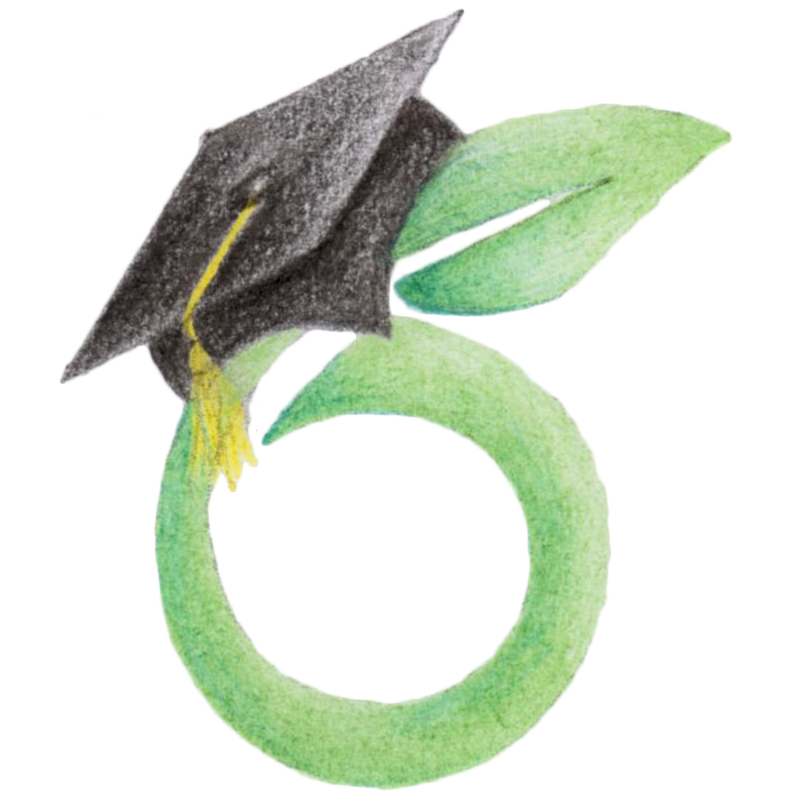
\includegraphics[width=0.3\textwidth]{overleaf.png}}
  \hfill
  \subfloat[latex]{
\includegraphics[width=0.3\textwidth]{latex.png}}
  \hfill
  \subfloat[github]{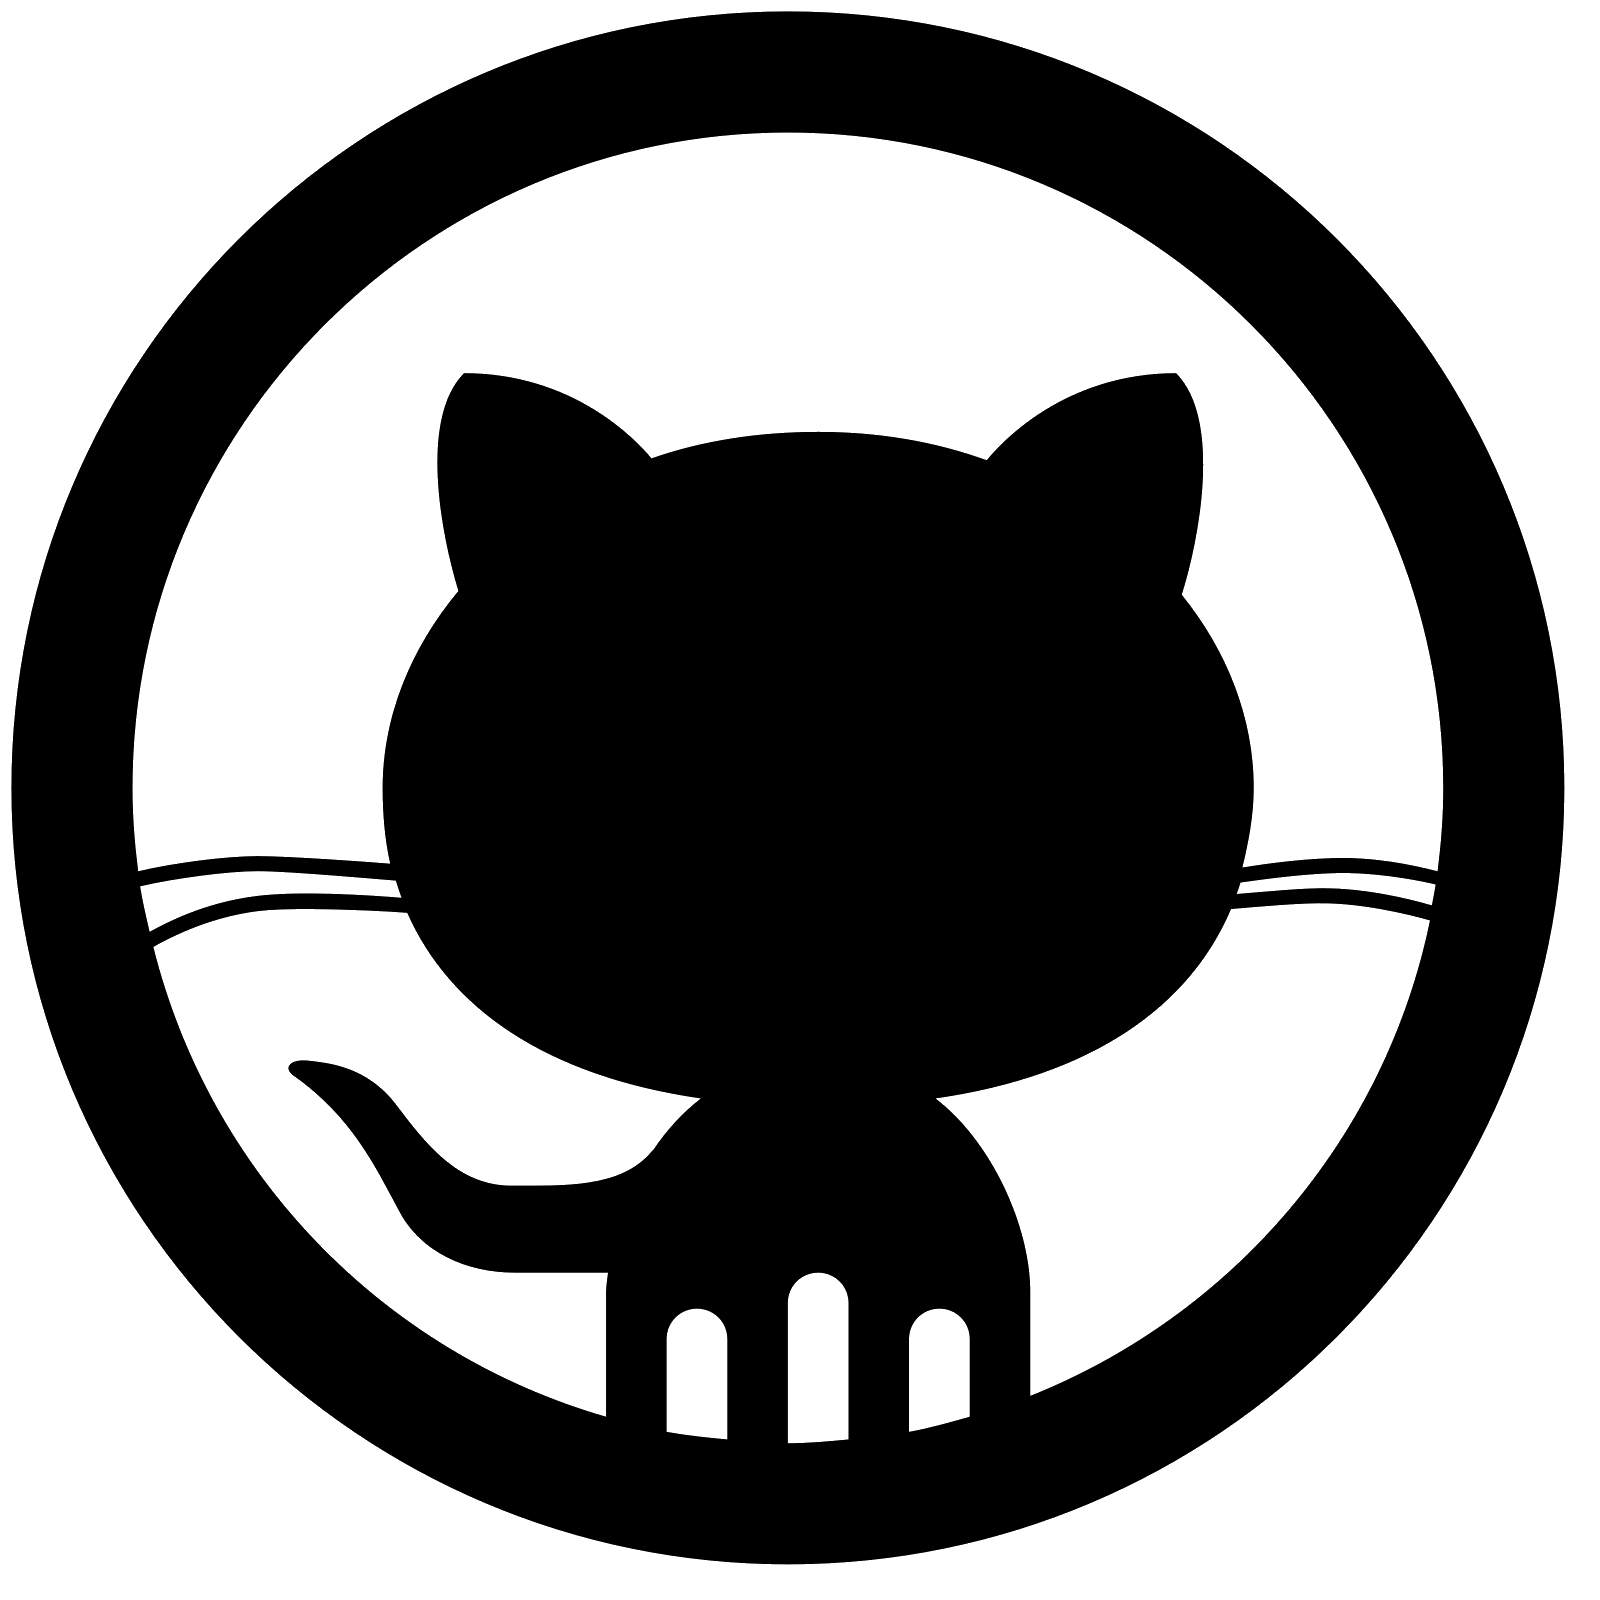
\includegraphics[width=0.3\textwidth]{github.png}}
  \legend{Google images}
  
\end{figure}

Integer tincidunt. Cras dapibus. Vivamus elementum semper nisi. Aenean vulputate eleifend tellus. Aenean leo ligula, porttitor eu, consequat vitae, eleifend ac, enim. Aliquam lorem ante, dapibus in, viverra quis, feugiat a, tellus. Phasellus viverra nulla ut metus varius laoreet. Quisque rutrum. Aenean imperdiet. Etiam ultricies nisi vel augue. Curabitur ullamcorper ultricies nisi. Nam eget dui. Etiam rhoncus. Maecenas tempus, tellus eget condimentum rhoncus, sem quam semper libero, sit amet adipiscing sem neque sed ipsum. Nam quam nunc, blandit vel, luctus pulvinar, hendrerit id, lorem. Maecenas nec odio et ante tincidunt tempus. Donec vitae sapien ut libero venenatis faucibus. Nullam quis ante. Etiam sit amet orci eget eros faucibus tincidunt. Duis leo. Sed fringilla mauris sit amet nibh. Donec sodales sagittis magna. Sed consequat, leo eget bibendum sodales, augue velit cursus nunc,

\subsection{Tabelas e Quadros}

Segue exemplos de como usar tabelas e quadros.

\begin{table}[ht]
  \caption{Faixa etária dos alunos (número e proporção) do Curso de Saneamento do Ifes – Campus Vitória no no de 2016.}
  \centering

  \begin{tabular}{ccc}
    \hline
    \bfseries Faixa Etária & \bfseries Número & Porcentagem\\
    \hline
    18 a 25 & 7 & 25,7 \\
    26 a 30 & 25 & 70,3 \\
    31 a 40 & 2 & 3,0 \\
    40 a 50 & 1 & 1,0 \\
    + de 50 & - & - \\
    \hline
    Total & 35 & 100 \\
    \hline
  \end{tabular}

  \source
\end{table}
  
\begin{quadro}[ht]
  \caption{Configuração de microcomputador XP.}
  \centering
  
  \resizebox{\textwidth}{!}{%
  \begin{tabular}{ll}
    \hline
    \bfseries Elemento & \bfseries Especificações\\
    \hline
    1 CD & CD + Disk Driver para apenas uma entrada de disquete \\
    Kit de multimídia 8X & Kit com placa de som, caixas, microfone, CD-ROM com velocidade 8X e títulos \\
    8 Mb RAM & Quantidade de memória RAM (ver memória) \\
    66 Mhz & Velocidade do computador \\
    PC 486 DX/2 & Tipo e modelo do computador \\
    840 Mb HD & Capacidade de armazenamento do computador \\
    \hline
  \end{tabular}}

  \legend{Barbosa (1999 apud UFES, 2004)}
\end{quadro}

\subsubsection{Teste com referências}

\begin{itemize}%[nosep]
  \item Citando o autor: \citeonline{Goodfellow2016}
  \item Citando o livro: \cite{Goodfellow2016}
  \item Citando o artigo: \cite{FernandezCaballero2016}
\end{itemize}
    
\subsubsubsection{Equações e Códigos}

O Teorema de Pitágoras é dado por:

\begin{equation}
	a^{2}= b^{2}+c^{2}
\end{equation}
  
Exemplo de código de programação:
  
\lstinputlisting[language=Python, caption=Perceptron]{algoritmos/perceptron.py}
    
  % --------------------------------------------------- %
  % ELEMENTOS POS-TEXTUAIS %
  % --------------------------------------------------- %

  \postextual
  
  % Referencias Bibliográficas
  \bibliographystyle{abntex2-alf} % Autor-Data
  \bibliography{bibliografia}
    
  % Apêndices
  \begin{apendicesenv}
    \chapter{Explicação}

É um elemento opcional. É um documento elaborado pelo próprio autor com o objetivo de completar sua argumentação, sem que haja prejuízo para a unidade do trabalho (ASSOCIAÇÃO BRASILEIRA DE NORMAS TÉCNICAS, 2011b. Deve ser precedido da palavra APÊNDICE (ex:APÊNDICE A, APÊNDICE B), identificado por letras maiúsculas consecutivas, travessão e pelo respectivo título. 
  \end{apendicesenv}

  % Anexos
  \begin{anexosenv}
    \chapter{Explicação}

É um elemento opcional. Não é elaborado pelo próprio autor mas sim por outras pessoas e constitui-se de suportes elucidativos e ilustrativos importantes para a compreensão do texto (ASSOCIAÇÃO BRASILEIRA DE NORMAS TÉCNICAS, 2011b). Havendo mais de um anexo, sua identificação deve ser feita por letra maiúscula ou algarismo arábico (ex:ANEXO A, ANEXO B), identificado por letras maiúsculas consecutivas,travessão e pelo respectivo título. 
    \chapter{{\normalfont EasyReview}}

\lstset{
		keywordstyle=\bfseries\color{purple!60!black},
		commentstyle=\itshape\color{green!40!black},
% 		identifierstyle=\itshape,
		stringstyle=\itshape,
		showstringspaces=false,
		escapeinside={\%*}{*)},
		columns=flexible,
		breaklines=true,
breakindent=0pt}

\renewcommand\lstlistingname{Example}
\newcommand{\keyword}[1]{\textbf{\color{purple!60!black}{#1}}}

% ------
\textbf{\uppercase {The alert command}}

% ------
Command intended to claim author's attention to a given part of the text. In the following, it is possible to see an example:

\begin{center}
\begin{minipage}[ht]{0.45\textwidth}
\begin{lstlisting}[language=tex]
A text without the alert command. %*\keyword{$\backslash$alert}*){A text with the alert command}.
\end{lstlisting}
\end{minipage}
\hspace{10pt}
\begin{minipage}[ht]{0.45\textwidth}
A text without the alert command. \alert{A text with the alert command}.
\end{minipage}
\end{center}

% ------
\textbf{\uppercase {The highlight command}}

% ------
Command intended to claim author's attention to a given part of the text in a different to the ``alert'' command. In the following, it is possible to see an example:

\begin{center}
\begin{minipage}[ht]{0.45\textwidth}
\begin{lstlisting}[language=tex]
A text without the highlight command. %*\keyword{$\backslash$highlight}*){A text with the highlight command}.
\end{lstlisting}
\end{minipage}
\hspace{10pt}
\begin{minipage}[ht]{0.45\textwidth}
A text without the highlight command. \highlight{A text with the highlight command}.
\end{minipage}
\end{center}

% ------
\textbf{\uppercase {The remove command}}

% ------
Command which an author suggest to remove a given part of the text. In the following, it is possible to see an example:

\begin{center}
\begin{minipage}[ht]{0.45\textwidth}
\begin{lstlisting}[language=tex]
This text is not to be removed. %*\keyword{$\backslash$remove}*){This text is to be removed}.
\end{lstlisting}
\end{minipage}
\hspace{10pt}
\begin{minipage}[ht]{0.45\textwidth}
This text is not to be removed. \remove{This text is to be removed}.
\end{minipage}
\end{center}

% ------
\textbf{\uppercase {The add command}}

% ------
Command which an author suggest to add new text in a given part of the text. In the following, it is possible to see an example:

\begin{center}
\begin{minipage}[ht]{0.45\textwidth}
\begin{lstlisting}[language=tex]
This text was already in the text. %*\keyword{$\backslash$add}*){This text is been added now}.
\end{lstlisting}
\end{minipage}
\hspace{10pt}
\begin{minipage}[ht]{0.45\textwidth}
This text was already in the text. \add{This text is been added now}.
\end{minipage}
\end{center}

% ------
\textbf{\uppercase {The replace/substitute command}}

% ------
Both commands are equivalent. It shall be used when an author suggest to replace a given part of the text for a newer one. In the following, it is possible to see an example:

\begin{center}
\begin{minipage}[ht]{0.45\textwidth}
\begin{lstlisting}[language=tex]
%*\keyword{$\backslash$replace}*){This part of the text needs to be replaced}{for this newer part of the text}.
\end{lstlisting}
\end{minipage}
\hspace{10pt}
\begin{minipage}[ht]{0.45\textwidth}
\replace{This part of the text needs to be replaced}{for this newer part of the text}.
\end{minipage}
\end{center}

% ------
\textbf{\uppercase {The commentreview command}}

% ------
Command intended to claim author's attention to a given part of the text, giving some comments to provide more information. In the following, it is possible to see an example:

\begin{center}
\begin{minipage}[ht]{0.45\textwidth}
\begin{lstlisting}[language=tex]
%*\keyword{$\backslash$commentreview}*){This text will receive a comment.}{This is the comment I have!}.
\end{lstlisting}
\end{minipage}
\hspace{10pt}
\begin{minipage}[ht]{0.45\textwidth}
\commentreview{This text will receive a comment.}{This is the comment I have!}.
\end{minipage}
\end{center}
  \end{anexosenv}

  % Índice Remissivo
  \phantompart
  \printindex

\end{document}